\documentclass[10pt, aspectratio=169]{beamer}
\usepackage{ifdraft}
\usepackage[backend=biber, language=english, style=authortitle-comp]{biblatex}

\usepackage{hiromacros}
\usepackage{fontspec}
\setmainfont{texgyrepagella}[
  Extension = .otf,
  UprightFont = *-regular,
  BoldFont = *-bold,
  ItalicFont = *-italic,
  BoldItalicFont = *-bolditalic,
  ]
\usepackage{unicode-math}
\usepackage[english]{babel}
\usepackage[justification=centering]{caption}
\usepackage[list=true, font=small,
labelformat=brace, position=top]{subcaption}
\usepackage[tbtags]{mathtools}
\usepackage{amssymb}
\usepackage{physics}
\usepackage{cleveref}
\usepackage{graphicx}

\usepackage{appendixnumberbeamer}
\graphicspath{ {./figs/} {./figs/drawings} }
\usepackage{tikz}
\usepackage{pgfplots}
\usetikzlibrary{calc,matrix,intersections,fillbetween}
% Plots
\usepackage{tikz}
\usepackage{pgfplots}
\usepackage{tikzscale}

\usetikzlibrary{external}
\tikzexternalize

\usetikzlibrary{arrows.meta}
\usetikzlibrary{backgrounds}
\usepgfplotslibrary{patchplots}
\usepgfplotslibrary{fillbetween}
\pgfplotsset{%
    layers/standard/.define layer set={%
        background,axis background,axis grid,axis ticks,axis lines,axis tick labels,pre main,main,axis descriptions,axis foreground%
    }{
        grid style={/pgfplots/on layer=axis grid},%
        tick style={/pgfplots/on layer=axis ticks},%
        axis line style={/pgfplots/on layer=axis lines},%
        label style={/pgfplots/on layer=axis descriptions},%
        legend style={/pgfplots/on layer=axis descriptions},%
        title style={/pgfplots/on layer=axis descriptions},%
        colorbar style={/pgfplots/on layer=axis descriptions},%
        ticklabel style={/pgfplots/on layer=axis tick labels},%
        axis background@ style={/pgfplots/on layer=axis background},%
        3d box foreground style={/pgfplots/on layer=axis foreground},%
    },
}
\pgfplotsset{
colormap={plots1}{rgb(0.00000000)=(0.00146200,0.00046600,0.01386600)
rgb(0.00392157)=(0.00226700,0.00127000,0.01857000)
rgb(0.00784314)=(0.00329900,0.00224900,0.02423900)
rgb(0.01176471)=(0.00454700,0.00339200,0.03090900)
rgb(0.01568627)=(0.00600600,0.00469200,0.03855800)
rgb(0.01960784)=(0.00767600,0.00613600,0.04683600)
rgb(0.02352941)=(0.00956100,0.00771300,0.05514300)
rgb(0.02745098)=(0.01166300,0.00941700,0.06346000)
rgb(0.03137255)=(0.01399500,0.01122500,0.07186200)
rgb(0.03529412)=(0.01656100,0.01313600,0.08028200)
rgb(0.03921569)=(0.01937300,0.01513300,0.08876700)
rgb(0.04313725)=(0.02244700,0.01719900,0.09732700)
rgb(0.04705882)=(0.02579300,0.01933100,0.10593000)
rgb(0.05098039)=(0.02943200,0.02150300,0.11462100)
rgb(0.05490196)=(0.03338500,0.02370200,0.12339700)
rgb(0.05882353)=(0.03766800,0.02592100,0.13223200)
rgb(0.06274510)=(0.04225300,0.02813900,0.14114100)
rgb(0.06666667)=(0.04691500,0.03032400,0.15016400)
rgb(0.07058824)=(0.05164400,0.03247400,0.15925400)
rgb(0.07450980)=(0.05644900,0.03456900,0.16841400)
rgb(0.07843137)=(0.06134000,0.03659000,0.17764200)
rgb(0.08235294)=(0.06633100,0.03850400,0.18696200)
rgb(0.08627451)=(0.07142900,0.04029400,0.19635400)
rgb(0.09019608)=(0.07663700,0.04190500,0.20579900)
rgb(0.09411765)=(0.08196200,0.04332800,0.21528900)
rgb(0.09803922)=(0.08741100,0.04455600,0.22481300)
rgb(0.10196078)=(0.09299000,0.04558300,0.23435800)
rgb(0.10588235)=(0.09870200,0.04640200,0.24390400)
rgb(0.10980392)=(0.10455100,0.04700800,0.25343000)
rgb(0.11372549)=(0.11053600,0.04739900,0.26291200)
rgb(0.11764706)=(0.11665600,0.04757400,0.27232100)
rgb(0.12156863)=(0.12290800,0.04753600,0.28162400)
rgb(0.12549020)=(0.12928500,0.04729300,0.29078800)
rgb(0.12941176)=(0.13577800,0.04685600,0.29977600)
rgb(0.13333333)=(0.14237800,0.04624200,0.30855300)
rgb(0.13725490)=(0.14907300,0.04546800,0.31708500)
rgb(0.14117647)=(0.15585000,0.04455900,0.32533800)
rgb(0.14509804)=(0.16268900,0.04355400,0.33327700)
rgb(0.14901961)=(0.16957500,0.04248900,0.34087400)
rgb(0.15294118)=(0.17649300,0.04140200,0.34811100)
rgb(0.15686275)=(0.18342900,0.04032900,0.35497100)
rgb(0.16078431)=(0.19036700,0.03930900,0.36144700)
rgb(0.16470588)=(0.19729700,0.03840000,0.36753500)
rgb(0.16862745)=(0.20420900,0.03763200,0.37323800)
rgb(0.17254902)=(0.21109500,0.03703000,0.37856300)
rgb(0.17647059)=(0.21794900,0.03661500,0.38352200)
rgb(0.18039216)=(0.22476300,0.03640500,0.38812900)
rgb(0.18431373)=(0.23153800,0.03640500,0.39240000)
rgb(0.18823529)=(0.23827300,0.03662100,0.39635300)
rgb(0.19215686)=(0.24496700,0.03705500,0.40000700)
rgb(0.19607843)=(0.25162000,0.03770500,0.40337800)
rgb(0.20000000)=(0.25823400,0.03857100,0.40648500)
rgb(0.20392157)=(0.26481000,0.03964700,0.40934500)
rgb(0.20784314)=(0.27134700,0.04092200,0.41197600)
rgb(0.21176471)=(0.27785000,0.04235300,0.41439200)
rgb(0.21568627)=(0.28432100,0.04393300,0.41660800)
rgb(0.21960784)=(0.29076300,0.04564400,0.41863700)
rgb(0.22352941)=(0.29717800,0.04747000,0.42049100)
rgb(0.22745098)=(0.30356800,0.04939600,0.42218200)
rgb(0.23137255)=(0.30993500,0.05140700,0.42372100)
rgb(0.23529412)=(0.31628200,0.05349000,0.42511600)
rgb(0.23921569)=(0.32261000,0.05563400,0.42637700)
rgb(0.24313725)=(0.32892100,0.05782700,0.42751100)
rgb(0.24705882)=(0.33521700,0.06006000,0.42852400)
rgb(0.25098039)=(0.34150000,0.06232500,0.42942500)
rgb(0.25490196)=(0.34777100,0.06461600,0.43021700)
rgb(0.25882353)=(0.35403200,0.06692500,0.43090600)
rgb(0.26274510)=(0.36028400,0.06924700,0.43149700)
rgb(0.26666667)=(0.36652900,0.07157900,0.43199400)
rgb(0.27058824)=(0.37276800,0.07391500,0.43240000)
rgb(0.27450980)=(0.37900100,0.07625300,0.43271900)
rgb(0.27843137)=(0.38522800,0.07859100,0.43295500)
rgb(0.28235294)=(0.39145300,0.08092700,0.43310900)
rgb(0.28627451)=(0.39767400,0.08325700,0.43318300)
rgb(0.29019608)=(0.40389400,0.08558000,0.43317900)
rgb(0.29411765)=(0.41011300,0.08789600,0.43309800)
rgb(0.29803922)=(0.41633100,0.09020300,0.43294300)
rgb(0.30196078)=(0.42254900,0.09250100,0.43271400)
rgb(0.30588235)=(0.42876800,0.09479000,0.43241200)
rgb(0.30980392)=(0.43498700,0.09706900,0.43203900)
rgb(0.31372549)=(0.44120700,0.09933800,0.43159400)
rgb(0.31764706)=(0.44742800,0.10159700,0.43108000)
rgb(0.32156863)=(0.45365100,0.10384800,0.43049800)
rgb(0.32549020)=(0.45987500,0.10608900,0.42984600)
rgb(0.32941176)=(0.46610000,0.10832200,0.42912500)
rgb(0.33333333)=(0.47232800,0.11054700,0.42833400)
rgb(0.33725490)=(0.47855800,0.11276400,0.42747500)
rgb(0.34117647)=(0.48478900,0.11497400,0.42654800)
rgb(0.34509804)=(0.49102200,0.11717900,0.42555200)
rgb(0.34901961)=(0.49725700,0.11937900,0.42448800)
rgb(0.35294118)=(0.50349300,0.12157500,0.42335600)
rgb(0.35686275)=(0.50973000,0.12376900,0.42215600)
rgb(0.36078431)=(0.51596700,0.12596000,0.42088700)
rgb(0.36470588)=(0.52220600,0.12815000,0.41954900)
rgb(0.36862745)=(0.52844400,0.13034100,0.41814200)
rgb(0.37254902)=(0.53468300,0.13253400,0.41666700)
rgb(0.37647059)=(0.54092000,0.13472900,0.41512300)
rgb(0.38039216)=(0.54715700,0.13692900,0.41351100)
rgb(0.38431373)=(0.55339200,0.13913400,0.41182900)
rgb(0.38823529)=(0.55962400,0.14134600,0.41007800)
rgb(0.39215686)=(0.56585400,0.14356700,0.40825800)
rgb(0.39607843)=(0.57208100,0.14579700,0.40636900)
rgb(0.40000000)=(0.57830400,0.14803900,0.40441100)
rgb(0.40392157)=(0.58452100,0.15029400,0.40238500)
rgb(0.40784314)=(0.59073400,0.15256300,0.40029000)
rgb(0.41176471)=(0.59694000,0.15484800,0.39812500)
rgb(0.41568627)=(0.60313900,0.15715100,0.39589100)
rgb(0.41960784)=(0.60933000,0.15947400,0.39358900)
rgb(0.42352941)=(0.61551300,0.16181700,0.39121900)
rgb(0.42745098)=(0.62168500,0.16418400,0.38878100)
rgb(0.43137255)=(0.62784700,0.16657500,0.38627600)
rgb(0.43529412)=(0.63399800,0.16899200,0.38370400)
rgb(0.43921569)=(0.64013500,0.17143800,0.38106500)
rgb(0.44313725)=(0.64626000,0.17391400,0.37835900)
rgb(0.44705882)=(0.65236900,0.17642100,0.37558600)
rgb(0.45098039)=(0.65846300,0.17896200,0.37274800)
rgb(0.45490196)=(0.66454000,0.18153900,0.36984600)
rgb(0.45882353)=(0.67059900,0.18415300,0.36687900)
rgb(0.46274510)=(0.67663800,0.18680700,0.36384900)
rgb(0.46666667)=(0.68265600,0.18950100,0.36075700)
rgb(0.47058824)=(0.68865300,0.19223900,0.35760300)
rgb(0.47450980)=(0.69462700,0.19502100,0.35438800)
rgb(0.47843137)=(0.70057600,0.19785100,0.35111300)
rgb(0.48235294)=(0.70650000,0.20072800,0.34777700)
rgb(0.48627451)=(0.71239600,0.20365600,0.34438300)
rgb(0.49019608)=(0.71826400,0.20663600,0.34093100)
rgb(0.49411765)=(0.72410300,0.20967000,0.33742400)
rgb(0.49803922)=(0.72990900,0.21275900,0.33386100)
rgb(0.50196078)=(0.73568300,0.21590600,0.33024500)
rgb(0.50588235)=(0.74142300,0.21911200,0.32657600)
rgb(0.50980392)=(0.74712700,0.22237800,0.32285600)
rgb(0.51372549)=(0.75279400,0.22570600,0.31908500)
rgb(0.51764706)=(0.75842200,0.22909700,0.31526600)
rgb(0.52156863)=(0.76401000,0.23255400,0.31139900)
rgb(0.52549020)=(0.76955600,0.23607700,0.30748500)
rgb(0.52941176)=(0.77505900,0.23966700,0.30352600)
rgb(0.53333333)=(0.78051700,0.24332700,0.29952300)
rgb(0.53725490)=(0.78592900,0.24705600,0.29547700)
rgb(0.54117647)=(0.79129300,0.25085600,0.29139000)
rgb(0.54509804)=(0.79660700,0.25472800,0.28726400)
rgb(0.54901961)=(0.80187100,0.25867400,0.28309900)
rgb(0.55294118)=(0.80708200,0.26269200,0.27889800)
rgb(0.55686275)=(0.81223900,0.26678600,0.27466100)
rgb(0.56078431)=(0.81734100,0.27095400,0.27039000)
rgb(0.56470588)=(0.82238600,0.27519700,0.26608500)
rgb(0.56862745)=(0.82737200,0.27951700,0.26175000)
rgb(0.57254902)=(0.83229900,0.28391300,0.25738300)
rgb(0.57647059)=(0.83716500,0.28838500,0.25298800)
rgb(0.58039216)=(0.84196900,0.29293300,0.24856400)
rgb(0.58431373)=(0.84670900,0.29755900,0.24411300)
rgb(0.58823529)=(0.85138400,0.30226000,0.23963600)
rgb(0.59215686)=(0.85599200,0.30703800,0.23513300)
rgb(0.59607843)=(0.86053300,0.31189200,0.23060600)
rgb(0.60000000)=(0.86500600,0.31682200,0.22605500)
rgb(0.60392157)=(0.86940900,0.32182700,0.22148200)
rgb(0.60784314)=(0.87374100,0.32690600,0.21688600)
rgb(0.61176471)=(0.87800100,0.33206000,0.21226800)
rgb(0.61568627)=(0.88218800,0.33728700,0.20762800)
rgb(0.61960784)=(0.88630200,0.34258600,0.20296800)
rgb(0.62352941)=(0.89034100,0.34795700,0.19828600)
rgb(0.62745098)=(0.89430500,0.35339900,0.19358400)
rgb(0.63137255)=(0.89819200,0.35891100,0.18886000)
rgb(0.63529412)=(0.90200300,0.36449200,0.18411600)
rgb(0.63921569)=(0.90573500,0.37014000,0.17935000)
rgb(0.64313725)=(0.90939000,0.37585600,0.17456300)
rgb(0.64705882)=(0.91296600,0.38163600,0.16975500)
rgb(0.65098039)=(0.91646200,0.38748100,0.16492400)
rgb(0.65490196)=(0.91987900,0.39338900,0.16007000)
rgb(0.65882353)=(0.92321500,0.39935900,0.15519300)
rgb(0.66274510)=(0.92647000,0.40538900,0.15029200)
rgb(0.66666667)=(0.92964400,0.41147900,0.14536700)
rgb(0.67058824)=(0.93273700,0.41762700,0.14041700)
rgb(0.67450980)=(0.93574700,0.42383100,0.13544000)
rgb(0.67843137)=(0.93867500,0.43009100,0.13043800)
rgb(0.68235294)=(0.94152100,0.43640500,0.12540900)
rgb(0.68627451)=(0.94428500,0.44277200,0.12035400)
rgb(0.69019608)=(0.94696500,0.44919100,0.11527200)
rgb(0.69411765)=(0.94956200,0.45566000,0.11016400)
rgb(0.69803922)=(0.95207500,0.46217800,0.10503100)
rgb(0.70196078)=(0.95450600,0.46874400,0.09987400)
rgb(0.70588235)=(0.95685200,0.47535600,0.09469500)
rgb(0.70980392)=(0.95911400,0.48201400,0.08949900)
rgb(0.71372549)=(0.96129300,0.48871600,0.08428900)
rgb(0.71764706)=(0.96338700,0.49546200,0.07907300)
rgb(0.72156863)=(0.96539700,0.50224900,0.07385900)
rgb(0.72549020)=(0.96732200,0.50907800,0.06865900)
rgb(0.72941176)=(0.96916300,0.51594600,0.06348800)
rgb(0.73333333)=(0.97091900,0.52285300,0.05836700)
rgb(0.73725490)=(0.97259000,0.52979800,0.05332400)
rgb(0.74117647)=(0.97417600,0.53678000,0.04839200)
rgb(0.74509804)=(0.97567700,0.54379800,0.04361800)
rgb(0.74901961)=(0.97709200,0.55085000,0.03905000)
rgb(0.75294118)=(0.97842200,0.55793700,0.03493100)
rgb(0.75686275)=(0.97966600,0.56505700,0.03140900)
rgb(0.76078431)=(0.98082400,0.57220900,0.02850800)
rgb(0.76470588)=(0.98189500,0.57939200,0.02625000)
rgb(0.76862745)=(0.98288100,0.58660600,0.02466100)
rgb(0.77254902)=(0.98377900,0.59384900,0.02377000)
rgb(0.77647059)=(0.98459100,0.60112200,0.02360600)
rgb(0.78039216)=(0.98531500,0.60842200,0.02420200)
rgb(0.78431373)=(0.98595200,0.61575000,0.02559200)
rgb(0.78823529)=(0.98650200,0.62310500,0.02781400)
rgb(0.79215686)=(0.98696400,0.63048500,0.03090800)
rgb(0.79607843)=(0.98733700,0.63789000,0.03491600)
rgb(0.80000000)=(0.98762200,0.64532000,0.03988600)
rgb(0.80392157)=(0.98781900,0.65277300,0.04558100)
rgb(0.80784314)=(0.98792600,0.66025000,0.05175000)
rgb(0.81176471)=(0.98794500,0.66774800,0.05832900)
rgb(0.81568627)=(0.98787400,0.67526700,0.06525700)
rgb(0.81960784)=(0.98771400,0.68280700,0.07248900)
rgb(0.82352941)=(0.98746400,0.69036600,0.07999000)
rgb(0.82745098)=(0.98712400,0.69794400,0.08773100)
rgb(0.83137255)=(0.98669400,0.70554000,0.09569400)
rgb(0.83529412)=(0.98617500,0.71315300,0.10386300)
rgb(0.83921569)=(0.98556600,0.72078200,0.11222900)
rgb(0.84313725)=(0.98486500,0.72842700,0.12078500)
rgb(0.84705882)=(0.98407500,0.73608700,0.12952700)
rgb(0.85098039)=(0.98319600,0.74375800,0.13845300)
rgb(0.85490196)=(0.98222800,0.75144200,0.14756500)
rgb(0.85882353)=(0.98117300,0.75913500,0.15686300)
rgb(0.86274510)=(0.98003200,0.76683700,0.16635300)
rgb(0.86666667)=(0.97880600,0.77454500,0.17603700)
rgb(0.87058824)=(0.97749700,0.78225800,0.18592300)
rgb(0.87450980)=(0.97610800,0.78997400,0.19601800)
rgb(0.87843137)=(0.97463800,0.79769200,0.20633200)
rgb(0.88235294)=(0.97308800,0.80540900,0.21687700)
rgb(0.88627451)=(0.97146800,0.81312200,0.22765800)
rgb(0.89019608)=(0.96978300,0.82082500,0.23868600)
rgb(0.89411765)=(0.96804100,0.82851500,0.24997200)
rgb(0.89803922)=(0.96624300,0.83619100,0.26153400)
rgb(0.90196078)=(0.96439400,0.84384800,0.27339100)
rgb(0.90588235)=(0.96251700,0.85147600,0.28554600)
rgb(0.90980392)=(0.96062600,0.85906900,0.29801000)
rgb(0.91372549)=(0.95872000,0.86662400,0.31082000)
rgb(0.91764706)=(0.95683400,0.87412900,0.32397400)
rgb(0.92156863)=(0.95499700,0.88156900,0.33747500)
rgb(0.92549020)=(0.95321500,0.88894200,0.35136900)
rgb(0.92941176)=(0.95154600,0.89622600,0.36562700)
rgb(0.93333333)=(0.95001800,0.90340900,0.38027100)
rgb(0.93725490)=(0.94868300,0.91047300,0.39528900)
rgb(0.94117647)=(0.94759400,0.91739900,0.41066500)
rgb(0.94509804)=(0.94680900,0.92416800,0.42637300)
rgb(0.94901961)=(0.94639200,0.93076100,0.44236700)
rgb(0.95294118)=(0.94640300,0.93715900,0.45859200)
rgb(0.95686275)=(0.94690300,0.94334800,0.47497000)
rgb(0.96078431)=(0.94793700,0.94931800,0.49142600)
rgb(0.96470588)=(0.94954500,0.95506300,0.50786000)
rgb(0.96862745)=(0.95174000,0.96058700,0.52420300)
rgb(0.97254902)=(0.95452900,0.96589600,0.54036100)
rgb(0.97647059)=(0.95789600,0.97100300,0.55627500)
rgb(0.98039216)=(0.96181200,0.97592400,0.57192500)
rgb(0.98431373)=(0.96624900,0.98067800,0.58720600)
rgb(0.98823529)=(0.97116200,0.98528200,0.60215400)
rgb(0.99215686)=(0.97651100,0.98975300,0.61676000)
rgb(0.99607843)=(0.98225700,0.99410900,0.63101700)
rgb(1.00000000)=(0.98836200,0.99836400,0.64492400)},
}

\usetheme{default}
\usecolortheme{dolphin}
\usefonttheme{professionalfonts}
%\usepackage{newmathpx}
\institute[McGill] % (optional)
{
  McGill University
}

\setbeamertemplate{itemize items}[default]
\setbeamertemplate{enumerate items}[default]
\setbeamertemplate{blocks}[shadow=true]
\setbeamercolor{block title}{use=structure,bg=structure.fg!50, fg=white}
\setbeamercolor{block body}{use=structure,bg=structure.fg!10}

\AtBeginSection[]
{
   \begin{frame}
       \tableofcontents[currentsection]
   \end{frame}
}


\AtBeginSubsection[]
{
   \begin{frame}
       \tableofcontents[currentsubsection]
   \end{frame}
 }

\setbeamertemplate{footline}[frame number]
%\setbeamertemplate{bibliography item}{\insertbiblabel}

\usepackage{pgfpages}
% \setbeameroption{show notes on second screen}

\makeatletter
\def\beamer@framenotesbegin{% at beginning of slide
     \usebeamercolor[fg]{normal text}
      \gdef\beamer@noteitems{}%
      \gdef\beamer@notes{}%
}
\makeatother

% Plots
% \newcommand{\plot}[1]{%
%   \ifdraft{\includegraphics[draft=false]{#1.pdf}}{\input{./figs/#1.pgf}}}



\addbibresource{references.bib}
\synctex=1
\title{Research Update: Non-Markovian Quantum Walk, Finite Size, Finite Coupling Strength}

\author{Valentin Boettcher}
\titlegraphic{
  
\includegraphics[height=1cm]{figs/Logo_McGill.pdf}
}
\institute{McGill University, Montreal}
\date{18.01.2023}
\beamertemplatenavigationsymbolsempty

\begin{document}
\hypersetup{pageanchor=false}
\begin{frame}[plain]
  \titlepage
  %\includegraphics[width=3cm]{figs/Logo_TU_Dresden.pdf}
\end{frame}

%\hypersetup{pageanchor=true}
\pagenumbering{arabic}
\begin{frame}
  \tableofcontents
\end{frame}

\section{Starting Point}
\begin{frame}
  \frametitle{Model \footcite{Ricottone2020}}
  \begin{columns}
    \begin{column}{.6\linewidth}
      \begin{itemize}
      \item<1-> consider an SSH chain lattice with extra levels in each unit cell
        \only<2>{\begin{align*}
                   \label{eq:36}
                   H_{A} &= ∑_{m}ω_{A} \ketbra{A,m} \\
                   H_{\bar{A}} &=\begin{aligned}[t]
                                   Σ_{m}&(ω_{A} + ω)\ketbra{B,m} +\\
                                        &∑_{j}\bqty{ω_{j}\ketbra{j, k} + g_{j}
                                          \pqty{\ketbra{j,m}{B,m} + \hc}}
                                 \end{aligned}
                   \\
                   V&=∑_{m} v\pqty{\ketbra{A,m}{B,m} + u\ketbra{A,m}{B,m+1} + \hc}
                 \end{align*}}
               \only<3>{
                 \begin{align*}
                   \label{eq:35}
                   H_{A}(k) &= ω_{A} \ketbra{A,k} \\
                   H_{\bar{A}}(k) &=
                                    \begin{aligned}[t]
                                      (&ω_{A} + ω)\ketbra{B,k}\\+
                                      &∑_{j}\bqty{ω_{j}\ketbra{j, k} + g_{j}
                                      \pqty{\ketbra{j,k}{B,k} + \hc}}
                                    \end{aligned}
                   \\
                   V(k)&=\abs{v(k)}\pqty{\eu^{\iu ϕ(k)}\ketbra{A,k}{B,k} + \hc}
                 \end{align*}
               }
             \item<4-> to make calculations simpler: eliminate \(B\) sites
               \only<4>{\begin{equation}
                   \label{eq:37}
                   \begin{aligned}
                     H(k) =  ∑_{j}& \bqty{\tilde{ω}_{j} \ketbra{j, k}
                     + \pqty{\tilde{η}_{j}\ketbra{A,k}{j,k} + \hc}} \\
                     &\tilde{ω}_{A} \ketbra{j,k}
                   \end{aligned}
                 \end{equation}
               }
      \end{itemize}
    \end{column}
    \begin{column}{.4\linewidth}
      \begin{figure}
        \centering
        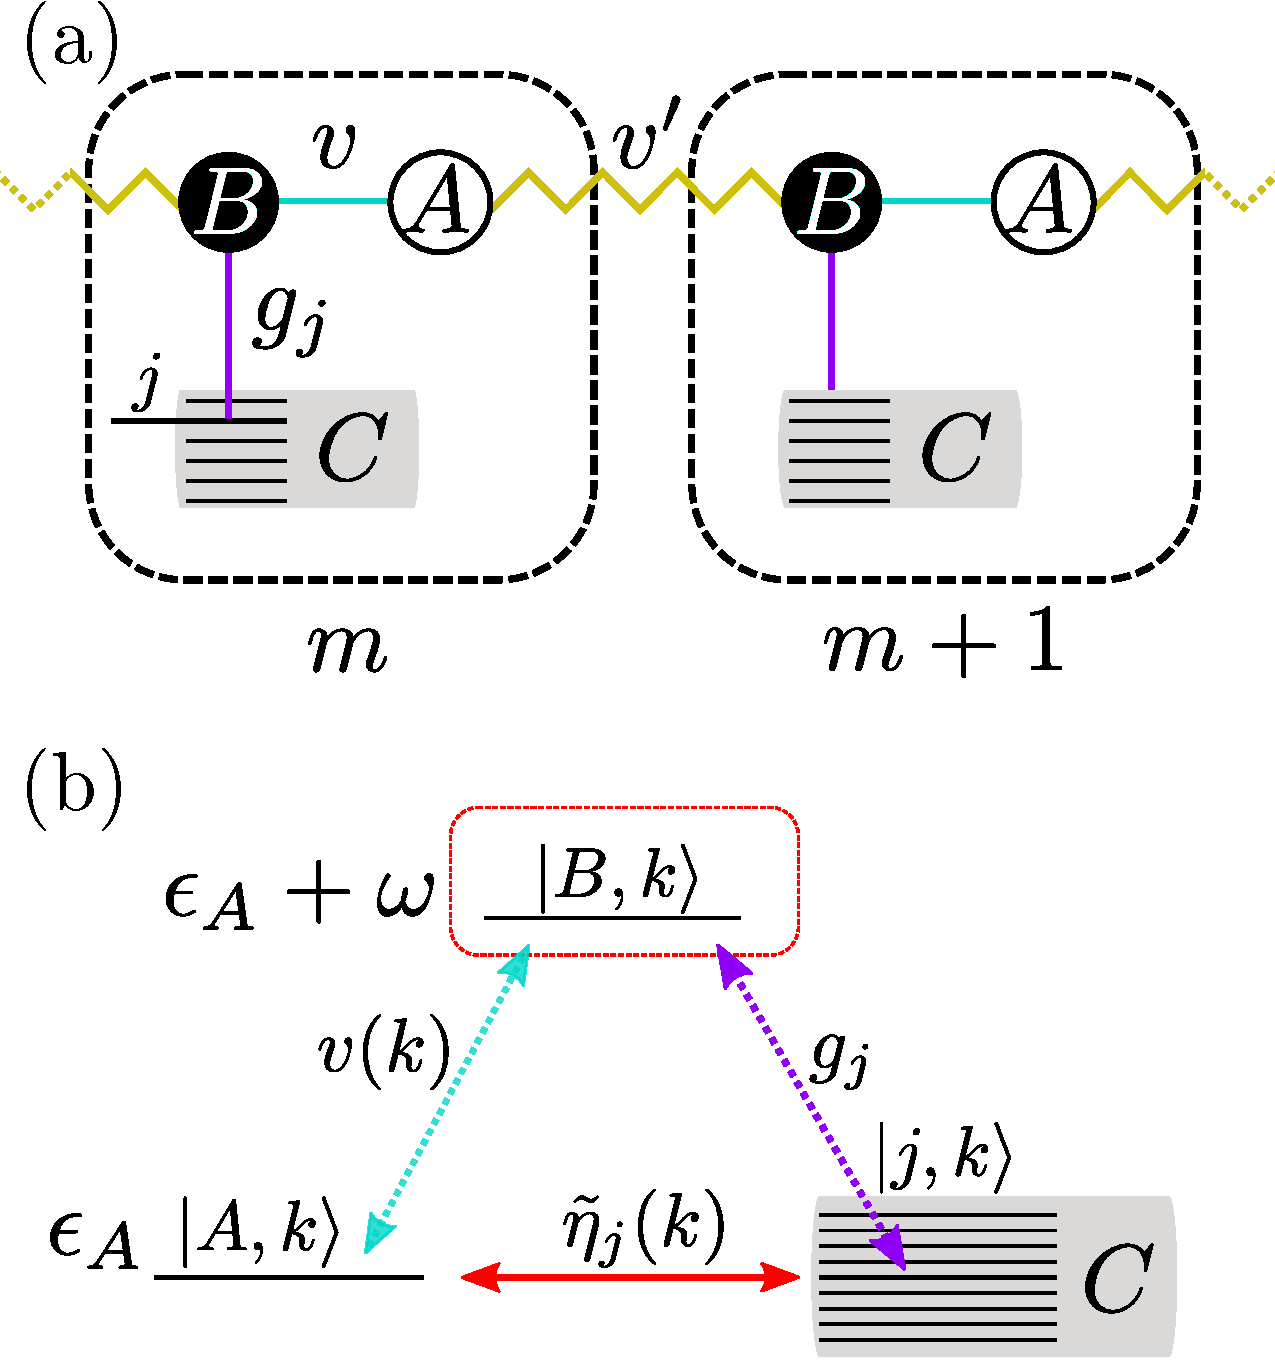
\includegraphics[width=\columnwidth]{figs/fig1.pdf}
      \end{figure}
    \end{column}
  \end{columns}
\end{frame}

\begin{frame}
  \frametitle{Observable}
  \begin{itemize}[<+->]
  \item the bare SSH model has a topoligical transition at
    \(v=v\prime\)
  \item consider average displacement before leaving the sublattice
    \begin{equation}
      \label{eq:38}
      \ev{m(t)} \equiv ∑_{m}m \pqty{1-ρ_{A,m}}  = ∑_{m}m \pqty{1-\abs{\braket{A,m}{ψ(t)}}^{2}}
    \end{equation}
  \item because of non-Markovianity: can oscillate \(\to\) consider
    time-average
    \begin{equation}
      \label{eq:39}
      \ev{m} \equiv \lim_{T\to ∞} \frac{1}{T}∫_{0}^{T}\ev{m(t)} \dd{t}
    \end{equation}

    \item  in momentum space \( \phi(k)=\arg [v(k)]=\arg \left[v\left(1+u e^{i k}\right)\right],\, u=\frac{v^{\prime}}{v} \)
\begin{equation}
  \label{eq:40}
  \ev{m} = ∫_{0}^{2π}(1-ρ_{A})\pdv{ϕ(k)}{k} \frac{\dd{k}}{2π}
\end{equation}
with
\begin{equation}
  \label{eq:41}
  ρ_{A}(k) = \lim_{T\to ∞}\frac{1}{T} ∫_{0}^{T}ρ_{A}(t, k)\dd{t} = \lim_{T\to
    ∞}\frac{1}{T} ∫_{0}^{T}\abs{\braket{A,k}{ψ(t)}}^{2}\dd{t}.
\end{equation}
  \end{itemize}
\end{frame}

\begin{frame}
  \frametitle{Spectral Densities}
  \begin{itemize}
  \item we need some values for the \(η_{j}\)
  \item in the continuum limit \(∑_{j}\abs{η_{j}}^{2} δ(ω-ω_{j}) =
    J(ω)\)
    \begin{equation}
      \label{eq:49}
      J(ω) =g_{0}^{2}\frac{α+1}{ω_{c}^{α+1}}
      \begin{dcases}
        ω^{α} & \mathrm{if}\, ω \leq ω_{c},\\
        0 & \mathrm{otherwise}.
      \end{dcases}
    \end{equation}
  \item we need the inverse choose \(η_{j}\) such that
    \begin{equation}
      \label{eq:48}
      ∫_{0}^{∞}f(ω)∑_{j}\abs{η_{j}}^{2} δ(ω-ω_{j})^{2}\dd{ω} =
      ∫_{0}^{∞}J(ω) f(ω)
    \end{equation}
  \item can be done more intricately, but for present purposes
    \begin{equation}
      \label{eq:1}
      \begin{aligned}
        ω_{j} &=\frac{j ω_{c}}{N} & η_{j}^{2} = J(ω_{j}) \frac{ω_{c}}{N}
      \end{aligned}
    \end{equation}
  \end{itemize}
\end{frame}

\begin{frame}{Behavior in Weak-Coupling Limit}
  \begin{columns}
    \begin{column}{.7\linewidth}
      \begin{itemize}
      \item for \(α<1\) \(ρ_{A}\to 0\), for \(α>0\) persistent
        oscillations
        \begin{equation}
          \ev{m} = ∫_{0}^{2π}(1-ρ_{A})\pdv{ϕ(k)}{k} \frac{\dd{k}}{2π}
        \end{equation}
        \begin{itemize}
        \item \(ρ_{A}=0\) \(\to\) \(\ev{m}\) is winding number \(\to\)
          universal behavior
        \item otherwise: any value of \(\ev{m}\) is possible
        \end{itemize}
      \end{itemize}
    \end{column}
    \begin{column}{.3\linewidth}
      \begin{figure}
        \centering
        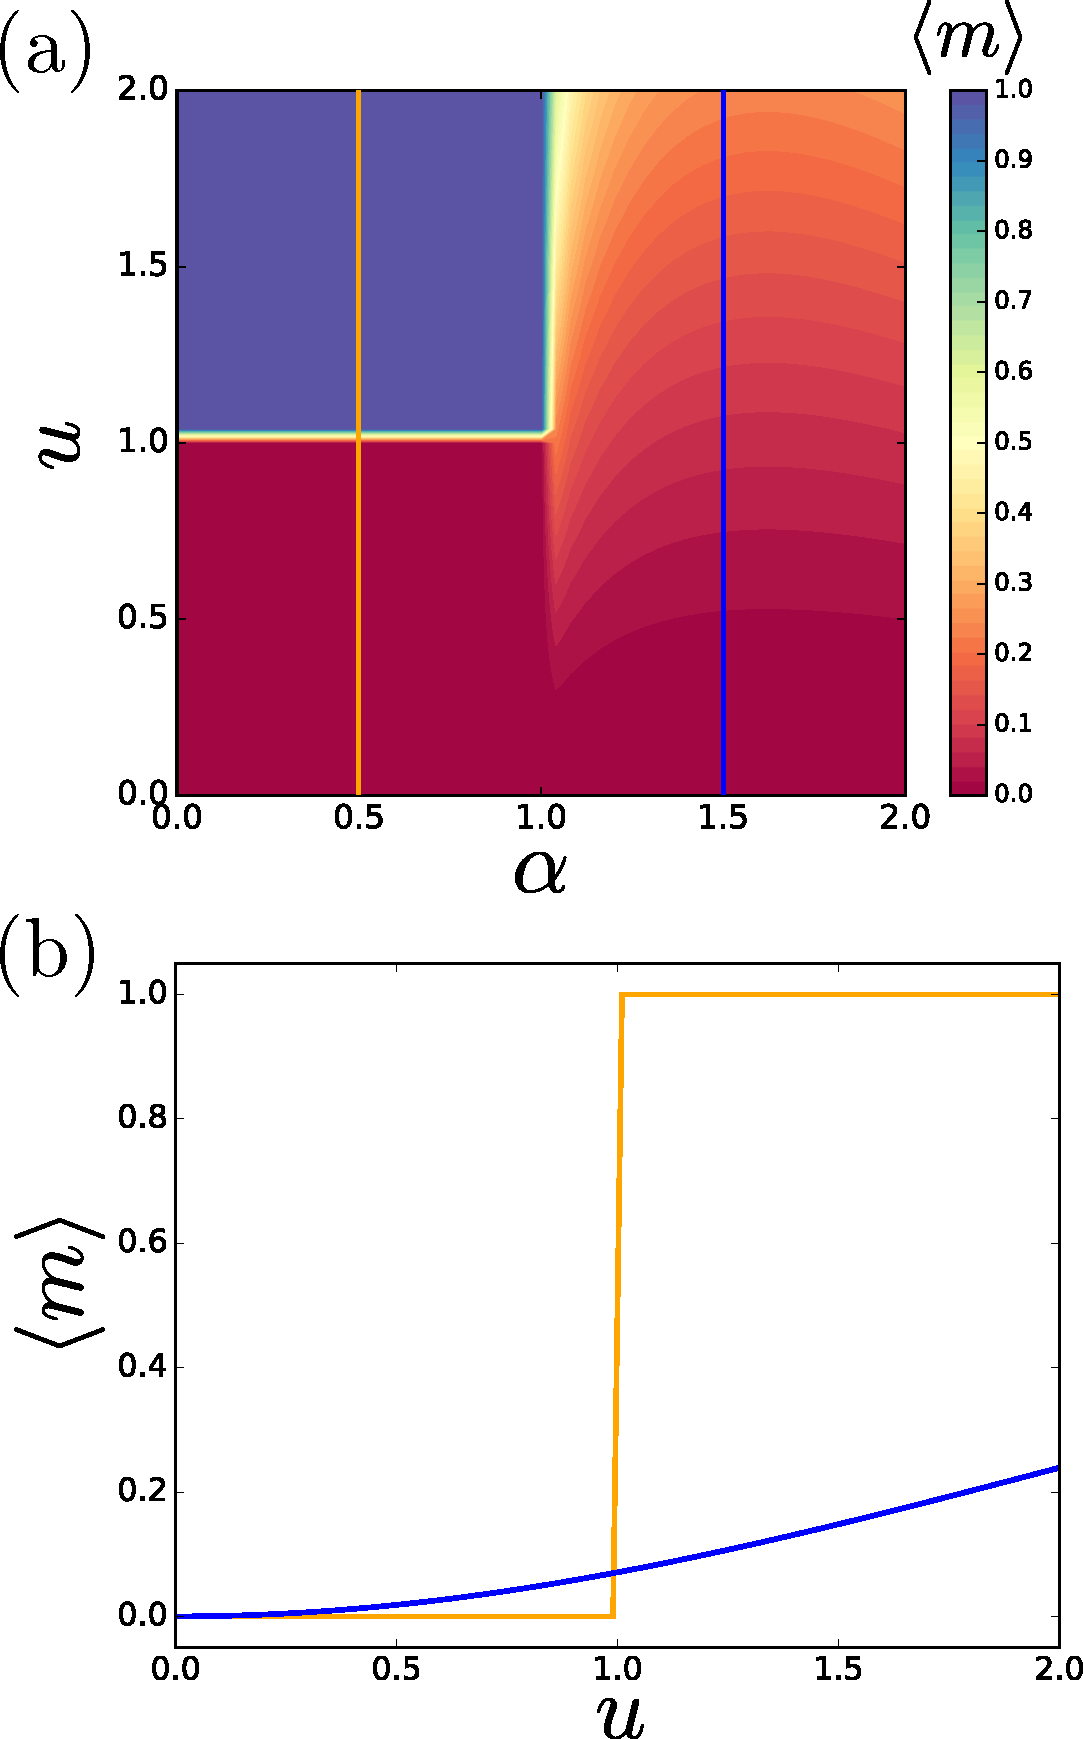
\includegraphics[width=\columnwidth]{figs/fig3.pdf}
      \end{figure}
    \end{column}
  \end{columns}
\end{frame}

\begin{frame}
  \frametitle{Solution in Weak Coupling Limit}
  \begin{itemize}
  \item can construct Master equation to second order in coupling
    \begin{equation}
      \label{eq:42}
      \dot{ρ}_{A}(k,t) = ∫_{0}^{t}Σ(k, t-t\prime) ρ_{A}(k, t\prime)
    \end{equation}
  \item solvable by Laplace transform, we only need long time limit
    though
    \begin{equation}
      \label{eq:44}
      {ρ}_{A}(k)=\lim_{T\to
        ∞}\frac{1}{T}∫_{0}^{∞}\eu^{-\frac{t}{T}}ρ_{A}(k,t)\dd{t} =
      \lim_{s\to 0} s \tilde{ρ}_{A}(k, s) = \eval{\bqty{\dv{s} \frac{1}{\tilde{ρ}_{A}(k,s)}}^{-1}}_{s=0}
    \end{equation}
  \item we find
    \begin{equation}
      \label{eq:47}
      ρ_{A}(k) = \frac{1}{1 + 2∑_{j}\frac{\abs{η_{j}}^{2}}{ω_{j}^{2}}} =
      \frac{1}{1+2 U_{A}}.
    \end{equation}
  \item \(U_{A}\) blows up for \(α < 1,\, N\to ∞\)
  \end{itemize}
\end{frame}

\begin{frame}
  \frametitle{The Conundrum}
  \begin{itemize}
  \item we would like to realize this model in a finite system
  \item coupling not necessarily vanishing (don't have infinite time)
  \item naive idea: just implement it numerically for a finite system
    and see what happens
    \begin{figure}[htp]
      \centering
      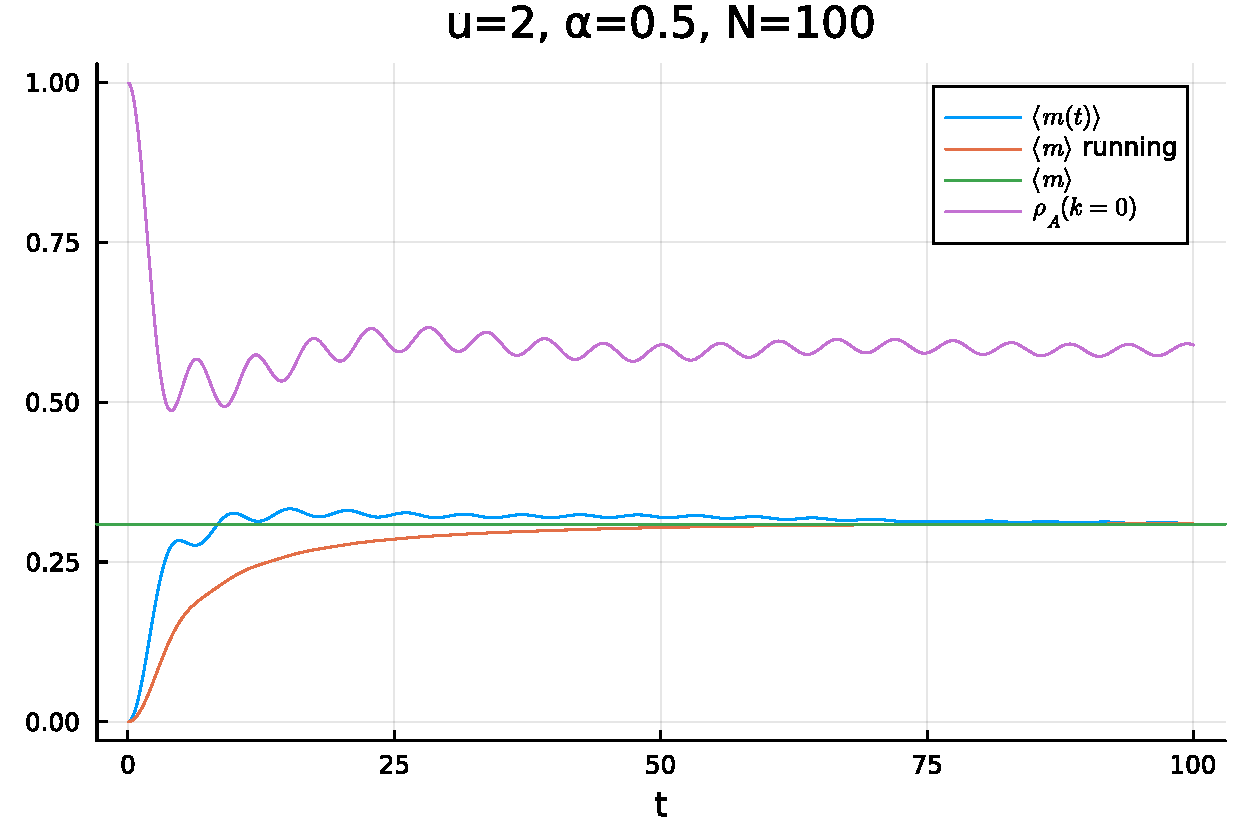
\includegraphics[width=.6\linewidth]{plots/overview_unshifted.tikz}
      \caption{\label{fig:unshifted_overview} A numerical simulation for
        \(g_{0}=10^{-2}\).}
    \end{figure}
  \end{itemize}
\end{frame}

\begin{frame}
  \frametitle{Problems}
  \begin{itemize}
  \item \(ρ_{A}\not\to 0\) \(\implies\) no universality
  \item finite \(N\) \(\implies\) recurrences

  \item played around with numerics: found that shifting \(ω_{A}\) can
    make \(ρ_{A}\to 0\)
  \item at finite strength: level repulsion shifts energy of the state
    that used to be \(\ket{A}\)
  \item destroys sensitivity for \(J(ω\to 0)\)
  \item shifting \(ω_{A}\) to compensate that Lamb shift can close the gap
    \begin{figure}[htp]
      \centering
      \begin{subfigure}[b]{0.45\columnwidth}
        \centering
        \includegraphics[width=\textwidth]{plots/spectrum_weak_couplign_limit.tikz}
      \end{subfigure}
      \begin{subfigure}[b]{0.45\columnwidth}
        \centering
        \includegraphics[width=\textwidth]{plots/spectrum_weak_shifted.tikz}
      \end{subfigure}
    \end{figure}
  \end{itemize}
\end{frame}

\begin{frame}
  \frametitle{Failed Idea: Brute-Forcing the Shift}
  \begin{itemize}
  \item a priori not clear how far to shift
  \item first approach: optimize \(ω_{A}\) to make gap in spectrum as
    small as possible
  \item leads to \(ρ_{A}\to 0\) regardless of \(α\)
  \item heuristic: first \(ω_{1}=ω_{c}/N\) \(\implies\) closing the
    gap \(ω_{1}\to 0\) \(\implies\) \(J(0)\neq 0 \implies ρ_{A}\to 0\)
  \end{itemize}
\end{frame}

\begin{frame}
  \frametitle{Exact Solution}
  \begin{itemize}
  \item Hamiltonian is very simple \(\implies\) exact solution
    actually exists
  \item define \(\ket{ψ} = α\ket{A} +
    ∑_{j}β_{j}\ket{j}\)
    \begin{equation}
      \label{eq:4}
      \dot{α} = -\iu ω_{A}α - ∫_{0}^{t} Κ(t-τ)α(τ) \dd{τ}
    \end{equation}
    with \(Κ(t-τ) = ∑_{j} \abs{η_{j}}^{2} \eu^{-\iu ω_{i}
      (t-τ)}\)
  \item Solution: Laplace-Transform
    \begin{equation}
      \label{eq:5}
      \begin{aligned}
        \tilde{α}(s) &= \frac{α(0)}{s+\iu ω_{A} + \tilde{Κ}(s)} &
                                                                  \tilde{Κ}(s) &= ∑_{j}\frac{\abs{η_{j}}^{2}}{s + \iu ω_{j}},
      \end{aligned}
    \end{equation}
  \item inversion: find poles \(ε_{i}\) (\(=\) finding the roots of the
    characteristic polynomial), calculate residues
    \begin{equation}
  \label{eq:6}
  α_{i} = \iu \lim_{ε\to ε_{i}} (ε-ε_{i}) \tilde{α}(-\iu ε) =
  \eval{\bqty{\dv{s} \frac{1}{\tilde{α}(-\iu s)}}^{-1}}_{s=ε_{i}} =
  \frac{α(0)}{1 + \tilde{Κ}'(-\iu ε_{i})} = \frac{α(0)}{1+U_{i}}
\end{equation}
  \end{itemize}
\end{frame}
\begin{frame}
  \frametitle{Mean Displacement}
  \begin{itemize}
  \item \(ρ_{A}(t) =
    \abs{α(t)}^{2} = ∑_{jk}α_{j}α_{k}^\ast \eu^{-\iu (ε_{j} - ε_{k})t}\)
    \(\rightarrow\) Laplace transform inversion does not commute
    \(\rightarrow\) need all poles, residues
  \item perturbation theory: have one state with great overlap with
    \(\ket{A}\) \(\rightarrow\) gives main contribution to
    \(\abs{α(t)}^{2}\)
  \item by choosing \(ω_{A}\) we can tune energy of this state
  \item let's set it to \(0\)
    \begin{equation}
      \label{eq:7}
      0 = \iu ω_{A} + \tilde{Κ}(0) \implies ω_{A} = ∑_{j}\frac{\abs{η_{j}}^{2}}{ε_{j}}
    \end{equation}

    \begin{equation}
      \label{eq:8}
      U_{A} = ∑_{j}\frac{\abs{η_{j}}^{2}}{ω_{j}^{2}} \implies ρ_{A}≥ \abs{α_{A}}^{2}
      = \frac{α(0)}{(1+U_{A})^{2}},
    \end{equation}
  \end{itemize}
\end{frame}


\begin{frame}{Comparison with Born}
  \begin{itemize}
  \item same expression for \(U_{A}\) \(\implies\) inherit behavior
  \item but \(ρ_{A}\) only compatible if \(U_{A} \ll 1 \implies
    (1+U_{A})^{2}\approx (1+2U_{A})\)

  \item also compatibility if \(U_{A}\to ∞\) in both cases and
    \(ω_{A}\to 0\)
  \item in continuum limit
    \begin{equation}
      \label{eq:10}
      ω_{A} = ∫_{0}^{ω_{c}}\frac{J(ω)}{ω} = J_{α}\frac{ω_{c}^{α}}{α}.
    \end{equation}
  \item using this in
    \begin{equation}
      \label{eq:12}
      ρ_{A}(k) = \frac{1}{1 + 2∑_{j}\frac{\abs{η_{j}}^{2}}{(ω_{j}-ω_{A})^{2}}}
    \end{equation}
    leads to \(ρ_{A}\to 1\, \forall α\)
  \item limits \(N\to ∞\) and \(g_{0}^{2}\to 0\) do not commute
  \item have to choose \(g_{0}\) for each \(N\) such that \(ω_{A}\to
    0\), then limit works
  \end{itemize}
\end{frame}

\begin{frame}{Formula for other Eigenvalues}
  Let us assume that \cref{eq:5} has a pole at
  \(-\iu (ω_{j}+δω_{j}) = -\iu ε_{j}\) with \(δω_{j}\ll ω_{j}\) so
  that
  \begin{equation}
    \label{eq:21}
    0 \overset{!}{=} ω_{j} + δω_{j} + ω_{A} -
    ∑_{l}\frac{\abs{η_{l}}^{2}}{ω_{l}-ω_{j}-δω_{j}} \approx ∑_{l\neq
      j}\frac{\abs{η_{l}}^{2}}{ω_{l}-ω_{j}} + δω_{j} ∑_{l\neq
      j}\frac{\abs{η_{l}}^{2}}{\pqty{ω_{l}-ω_{j}}^{2}} - \frac{\abs{η_{j}}^{2}}{δω_{j}},
  \end{equation}
  which can be solved for \(δω_{j}\)
  \begin{equation}
    \label{eq:22}
    δω_{j} = \frac{\sign{A_{j}}}{2(1+B_{j})} \bqty{\abs{A_{j}} -\sqrt{{A_{j}^{2}} +
        4(B_{j}+1)\abs{η_{j}}^{2}}}
  \end{equation}
  with
  \begin{equation}
    \label{eq:23}
    \begin{aligned}
      A_{j} &= ∑_{l\neq
              j}\frac{\abs{η_{l}}^{2}}{ω_{l}-ω_{j}} + ω_{j}-ω_{A} & B_{j} &=∑_{l\neq
                                                                            j}\frac{\abs{η_{l}}^{2}}{\pqty{ω_{l}-ω_{j}}^{2}}.
    \end{aligned}
  \end{equation}
\end{frame}

\begin{frame}
  \frametitle{Strong Coupling Limit}
  For \(∑_{j}\abs{η_{j}}^{2} \gg ω_{c}^{2}\) we can find an
  effective two-level system.

  \begin{figure}[htp]
    \centering
    \begin{subfigure}[b]{0.48\textwidth}
      \centering
      \includegraphics[width=\textwidth]{plots/spectrum_weak_couplign_limit.tikz}
    \end{subfigure}
    \begin{subfigure}[b]{0.48\textwidth}
      \centering
      \includegraphics[width=\textwidth]{plots/spectrum_stong_couplign_limit.tikz}
    \end{subfigure}
    \caption{\label{fig:spectrum_strong_coupling_limit} The spectrum of
      the model in \cref{fig:unshifted_overview} for two different
      coupling strengths. The bars show the overlap
      \(\abs{\braket{A}{E}}^{2}\) of the eigenstate \(\ket{E}\) at
      energy \(E\) with the \(\ket{A}\) state.}
  \end{figure}
\end{frame}
\begin{frame}
  \frametitle{Trivial Behavior of \(ρ_A\)}
  \begin{itemize}
  \item two eigenstates are complete basis of subspace that has
    overlap with \(\ket{A}\) level
  \item perfect oscillations between \(\ket{A}\) and some state
    support only in the bath \(ρ_{A}=1/2\)
  \end{itemize}
  \begin{columns}
    \begin{column}{.6\linewidth}
      \begin{figure}[htp]
        \centering
        \includegraphics[width=\columnwidth]{plots/strong_coupling_oscillations.tikz}
      \end{figure}
    \end{column}
    \begin{column}{.4\linewidth}
      \begin{equation}
        \label{eq:16}
        \ev{m} =
        \begin{cases}
          \frac{1}{2} & \mathrm{if}\, u>1,\\
          0 & \mathrm{if}\, u<1.
        \end{cases}
      \end{equation}
    \end{column}
  \end{columns}
\end{frame}

\begin{frame}
  \frametitle{Bath Size Requirements}
  \begin{itemize}
  \item assume \(N \sim 100\) and constant DOS \(η_{j}^{2} = J_{α}
    ω_{j}^{α}\) and \(ω_{j}=jω_{c}/N\)
  \item
  \end{itemize}
  \begin{equation}
    \label{eq:17}
    U_{A} = ∑_{j}\frac{η_{j}^{2}}{ω_{j}^{2}} = J_{α}
    \frac{ω_{C}}{N}∑_{j}{ω_{j}^{α-2}}= g_{0}^{2} \frac{α+1}{ω_{c}^{2}}
    N^{1-α} ∑_{j} j^{α-2}.
  \end{equation}
  For \(1/N\) sufficiently smaller than \(1\) we can approximate the sum
  in
  \cref{eq:17} as
  \begin{equation}
    \label{eq:18}
    N^{1-α} ∑_{j} j^{α-2} \approx \frac{g_{0}^{2} (α+1)}{ω_{c}^{2}} \pqty{N^{1-α}ζ(2-α) + \frac{1}{α-1}}.
  \end{equation}
  Demanding that \(ρ_{A}\approx \abs{α_{A}}^{2}\) takes on a particular
  value for a given \(α\) yields
  \begin{equation}
    \label{eq:19}
    N = \bqty{\pqty{\frac{ω_{c}^{2}}{g_{0}^{2}}\frac{\pqty{\abs{α_{A}}^{-1}-1}}{(α+1)}+\frac{1}{1-α}}\frac{1}{ζ(2-α)}}^{\frac{1}{1-α}}.
  \end{equation}
\end{frame}
\begin{frame}{How far away is the continuum limit?}
  \begin{figure}[tp]
    \centering
    \includegraphics[width=.5\linewidth]{plots/N_formula_surface.tikz}
    \caption{\label{fig:N_formula_surface} \Cref{eq:19} evaluated for
      \(g_{0}^{2}=0.05\) and \(ω_{c}=1\).  For \(α\lesssim 4\) we can
      expect relatively good results for \(\ev{m}\) for
      \(\mathcal{O}(100)\) bath levels.}
  \end{figure}
  \begin{itemize}
  \item \(α\approx 1\) gives limit
    \begin{equation}
      \label{eq:20}
      N \approx \pqty{ \frac{ω_{c}^{2}}{g_{0}^{2}}\pqty{\abs{α_{A}}^{-1}-1}\cdot
        \frac{1-α}{1+α}+1}^{\frac{1}{1-α}} \xrightarrow{α\to 1} \eu^{\frac{ω_{c}^{2}}{2g_{0}^{2}}\pqty{\abs{α_{A}}^{-1}-1}}
    \end{equation}
  \end{itemize}
\end{frame}

\begin{frame}{Mean Displacement with \(ω_{A}\) shift}
  \begin{itemize}
  \item \(k\) dependence \(\implies\) calculate \(ω_{A}\) for \(k=0\)
    \begin{itemize}
    \item as \(ω_{A}(k)≥ω_{A}(0)\) we will have \(ρ_{A}\to 0\)
      generically
    \item not the whole picture though \(\implies\) for \(u\) large
      variations in coupling strength
    \item note also: should normalize \(v (1+u) = v + v\prime\)
      remains constant
    \end{itemize}
  \end{itemize}
\end{frame}

\begin{frame}
    \begin{figure}
    \centering
    \includegraphics[width=.8\textwidth]{plots/overview_shifted.tikz}
    \caption{\label{fig:overview_shifted_many} With \(N=100\)
      bath levels and \(g_{0}^{2}=0.1\). The mean displacement approaches the universal
      value for finite times and the infinite time limit is not
      too far off.}
  \end{figure}
\end{frame}


\begin{frame}
    \begin{figure}
    \centering
    \includegraphics[width=.8\textwidth]{plots/overview_shifted_few.tikz}
  \end{figure}
\end{frame}

\begin{frame}
    \begin{figure}
    \centering
    \includegraphics[width=.8\textwidth]{plots/overview_shifted_few_windowed.tikz}
  \end{figure}
\end{frame}

\begin{frame}
  \begin{figure}[H]
  \centering
  \includegraphics[width=.8\linewidth]{plots/transition_u_graphs_wider.tikz}
  \caption{\label{fig:transition_u_graphs.tikz} \(\ev{m(t)}\)
    averaged over an interval \([0.5τ, 0.95τ]\) where \(τ\) is the
    recurrence time. The coupling strength was \(g_{0}^{2}=.05\) and
    \(N=100\) bath levels were used. This is on the same order of
    magnitude of what \cref{eq:19} would suggest, but windowing
    improves the result.}
\end{figure}
\end{frame}

\begin{frame}
  \begin{figure}[H]
    \centering
    \begin{subfigure}[t]{.49\linewidth}
      \includegraphics[width=\linewidth]{plots/phase_diag_100.tikz}
      \caption{With windowing.}
    \end{subfigure}
    \begin{subfigure}[t]{.49\linewidth}
      \includegraphics[width=\linewidth]{plots/phase_diag_100_nowindow.tikz}
      \caption{Without windowing. The phase diagram is slightly less
        crisp, but still acceptable.}
    \end{subfigure}
    \caption{\label{fig:fullphase}Full phase diagrams with the same
      parameters as \cref{fig:transition_u_graphs.tikz}.}
  \end{figure}
\end{frame}

\begin{frame}
  \begin{figure}[H]
    \centering
    \begin{subfigure}[t]{.49\linewidth}
      \includegraphics[width=\linewidth]{plots/phase_diag_100_nowindow_noshift.tikz}
      \caption{Without Lamb-Shift compensation. No universal values of
        \(\ev{m}\) are being reached.}
    \end{subfigure}
    \begin{subfigure}[t]{.49\linewidth}
      \includegraphics[width=\linewidth]{plots/phase_diag_10_strong.tikz}
      \caption{Without Lamb-Shift compensation in the strong coupling limit.}
    \end{subfigure}
    \caption{\label{fig:fullphase}Full phase diagrams with the same
      parameters as \cref{fig:transition_u_graphs.tikz}.}
  \end{figure}
\end{frame}
\end{document}

%%% Local Variables:
%%% mode: latex
%%% TeX-master: t
%%% TeX-output-dir: "output"
%%% TeX-engine: luatex
%%% End:
